\documentclass[a4paper,12pt,twoside]{book}
\usepackage[utf8]{inputenc}
\usepackage[T1]{fontenc}
\usepackage{fancyhdr}
\usepackage{float}
\usepackage{graphicx}
\graphicspath{ {figuras/} }

\title{Breve ensayo sobre el rompimiento de simetría y física de Higgs}
\author{Hernández Aceves Hugo}
\date{Viernes veinte de octubre de 2017}


\begin{document}
\maketitle
\thispagestyle{empty}
\tableofcontents
\pagenumbering{Roman}

\chapter{Resumen}\label{cap.resumen}
La ruptura espontánea de simetría es la pérdida de simetría de una lagrangiana respecto a un grupo. En la ruptura de simetría tienen lugar el surgimiento de nuevas partículas como bosones, debido al Mecanismo de Higgs.
El mecanismo de Higgs por su parte es el proceso en el que los bosones dan masa a las partículas interactuando con el campo de Higgs.
\chapter{Introducción}\label{cap.introduccion}
Para hablar del rompimiento espontáneo de simetría y mecanismo de Higgs es necesario al menos tener una remota idea de la física de partículas. La intención de este trabajo no es el de abordar ni siguiera a un nivel medianamente profundo este tema, pues sería imposible para cualquier ser humano entenderlo en un fin de semana, es por eso que en esta introducción fijaremos en la mente los elementos del modelo estándar de partículas y la física cuántica para poder tener una idea general al menos de lo que se está hablando.
En la teoría cuántica de campos de partículas elementales existen doce partículas subatómicas llamadas fermiones y divididas a su vez en dos grupos, Quarks y Leptones. Los Quarks son seis y tienen los siguientes extraños nombres: Up, Down, Charm, Strange, Top y Bottom, los quarks Up y Down se encuentran dentro de los bariones, particularmente en los neutrones y los protones, los demás quarks tienen un papel importante para explicar los fenómenos descubiertos en los aceleradores de partículas. Los leptones por su parte también son seis, tres de ellos tienen carga eléctrica, y son el muón, el tau y por supuesto el electrón, los otros tres restantes son los neutrinos que claramente son neutrales eléctricamente, que son similarmente: muón neutrino, tau neutrino y electrón neutrino. Con estos fermiones de construye el universo; con Up, Down y el electrón. Pero la forma en que estos interactúan entre sí está determinada por fuerzas relacionadas a otro tipo de partículas llamadas bosones.
Los bosones son probablemente cuatro: el fotón que es la partícula de la luz y de la fuerza electromagnética en general, los bosones w y z que generan una fuerza llamada fuerza nuclear débil, el gluón que genera una fuerza llamada fuerza nuclear fuerte y el hipotético gravitón, que generaría la fuerza gravitacional.
Debido a los bosones, en la naturaleza existen cuatro fuerzas que son llamadas fuerzas fundamentales, porque a diferencia de cualquier otra, tienen la propiedad de que no son el resultado de otras fuerzas, y son:
\begin{itemize}
\item Fuerza fundamental gravitatoria
\item Fuerza fundamental electromagnética
\item Fuerza fundamental fuerte
\item Fuerza fundamental débil

\end{itemize}

La fuerza fundamental gravitacional o interacción gravitatoria es la responsable de lo que denominamos comúnmente "\textit{gravedad}", es una fuerza de alcance largo pero es la más débil de todas, del orden de $10^{-40}$ veces la fuerza de la interacción fuerte, es de la que menos se conoce debido a su pequeñez.

La fuerza fundamental o interacción electromagnética es la responsable, claro, de la electricidad y el magnetismo, así como la luz y del hecho de que los electrones estén orbitando el núcleo atómico. También es una fuerza de alcance largo, pero a diferencia de la fuerza gravitacional, es alrededor de una centésima de la fuerza fuerte, se encarga de la atracción de partículas cargadas.

La fuerza fundamental fuerte es la más fuerte de todas y funciona a muy corto alcance, es responsable de unir a los quarks dentro de los protones y los neutrones.

La fuerza fundamental débil es sólo más fuerte que la gravedad y es la responsable de algunos tipos de radioactividad, es de corto al cance y al igual que la interacción fuerte, sólo tiene un efecto apreciable en distancias menores que la del tamaño de un protón.
\begin{center}
\textit{Aviso: Hasta este momento termina la parte del "ensayo" que tiene sentido, el siguiente capítulo deja ya de tener sentido,  es un esfuerzo de varios días por sintetizar algunos conceptos inentendibles (al menos para alguien que sólo sabe de mecánica clásica elemental) sobre temas bastante complejos. El texto recuperará en el capítulo de conclusión}
\end{center}


\chapter{Contenido}\label{cap.contenido}


\section{Ruptura espontánea de simetría}
Se dice que hay una ruptura espontánea de simetría SSB por sus siglas en inglés "spontaneous symmetry breaking" cuando en un sitema dado por alguna lagrangiana simétrica respecto a algún grupo de simetría entra en un estado de no simetría. Particularmente en la mecánica cuántica sucede en los medios uniformes que estén constituidos por un buen número de elementos. Las rupturas espontáneas se caracterizan por: la deformación del estado fundamental y una operación de simetría llevará de un estado fundamental al otro, de los estados fundamentales un único estado y todo un conjunto de ellos excitados son realizados dada una situación, la ruptura espontánease perde generalmente en temperaturas elevadas.
Para empezar, tenemos el Lagrangiano \\
$L_{0}=\partial^{\mu}\phi\partial_{\mu}\phi^{\dagger}-v(\phi\phi^{\dagger})$ \\
Análogamente cuando tenemos un superconductor  supondremos que el estado que minimiza V no es $\phi=0$, es decir $\phi_{0}\neq 0$, se dice aquí que la deformación es infinita y la simetría global está espontáneamente rota. Se elige \\
$v(\phi\phi^{\dagger}=\mu^{2}(\phi\phi^{\dagger})+\lambda(\phi\phi^{\dagger})^{2}+...$ \\
De este modo la energía del campo dse delimita desde $\lambda>0$. Esto depende del signo de $\lambda^{2}$
\begin{itemize}
\item $\lambda^{2}>0$. Aquí, los términos para V son mayores que cero y se puede ver el potencial como función de $\phi_{1}$ y $\phi_{1}$. Cuando $\phi(x)=0$ existe un mínimo para V, el rompimiento. Si consideramos $\lambda(\phi\phi^{\dagger})^{2}$ una perturbación, podemos entonces describirlo como el lagrangiano de Klein-Gordon.
\item $\lambda^{2}<0$. Aquí,V posee máximo local para $\phi(x)=0$ y en\\
$\phi(x)=\phi_{0}=(\frac{-\mu^{2}}{2\lambda})^{\frac{1}{2}}e^{i\Theta}$, $0\leq\Theta\leq2\pi$\\
un círculo de mínimo absoluto.
A continuación, una figura:
\begin{figure}[h]
\begin{center}
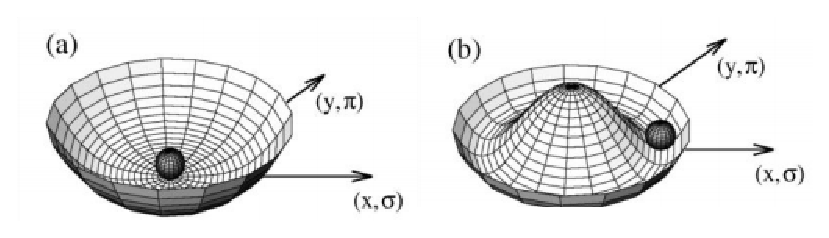
\includegraphics[scale=1]{imagen}
\caption{La simetría y su ruptura espontánea. a)Sistema simétrico estable. b)Sistema con solución asimétrica}
\label{fig:a}
\end{center}
\end{figure}


\end{itemize}


\section{Mecanismo de Higgs}
\textit{A continuación escribiremos un estracto de wikipedia con el fin de que queden varias páginas y se pueda apreciar el formato de numeración de página}

"En física de partículas, mecanismo de Higgs, también llamado como el mecanismo de Brout– Englert– Higgs o mecanismo de Englert- Brout- Higgs-G uralnik- Hagen- Kibble,1 es uno de los posibles mecanismos para producir la ruptura espontánea de simetría electrodébil en una teoría de gauge invariante. Permitió establecer la unificación entre la teoría electromagnética y la teoría nuclear débil, que se denominó Teoría del campo unificado, por la que obtendrían el premio Nobel en el año 19792 Steven Weinberg, Sheldon Lee Glashow y Abdus Salam.

El mecanismo de Higgs es el proceso que da masa a las partículas elementales. Las partículas ganan masa interactuando con el campo de Higgs que permea todo el espacio. Más precisamente, en una teoría de gauge, el mecanismo de Higgs dota con masa a los bosones de gauge a través de la absorción de los bosones de Nambu–Goldstone derivados de la ruptura espontánea de simetría.

La implementación más simple del mecanismo agrega un campo de Higgs extra a la teoría de gauge. La ruptura espontánea de la simetría local subyacente desencadena la conversión de los componentes de este campo de Higgs a bosones de Goldstone que interactúan (al menos algunos de ellos) con los demás campos de la teoría, con el fin de producir términos de masas para (al menos algunos de) los bosones de gauge. Este mecanismo también puede dejar detrás partículas escalares elementales (spin-0), conocidas como bosones de Higgs.

En el modelo estándar, la frase "mecanismo de Higgs" se refiere específicamente a la generación de masas para los bosones débiles de gauge, W, y Z a través de la simetría electrodébil.3

El mecanismo fue propuesto en 1962 por Philip Warren Anderson. El modelo relativista fue desarrollado en 1964 por tres grupos independientes: Robert Brout y Francois Englert; Peter Higgs; y Gerald Guralnik, C. R. Hagen y Tom Kibble. El 4 de julio de 2012, el Gran colisionador de hadrones (LHC) en el CERN anunció resultados consistentes con la partícula de Higgs, pero subrayó que son necesarias más pruebas para confirmar el mecanismo completo.
Este mecanismo también es conocido como mecanismo de Brout– Englert– Higgs, mecanismo de Higgs– Brout– Englert– Guralnik– Hagen– Kibble, o mecanismo de Anderson– Higgs. En 1964, fue inicialmente propuesto por Robert Brout y François Englert,4 e independientemente por Peter Higgs5 y por Gerald Guralnik, C. R. Hagen, y Tom Kibble.6 Fue inspirado en la Teoría BCS de rompimiento de simetría en superconductividad basado en Teoría Ginzburg-Landau, los trabajos de la estructura del vacío de Yoichiro Nambu, y las ideas de Philip Anderson según las cuales la superconductividad podía ser relevante en la relatividad, el electromagnetismo y otros fenómenos clásicos. El nombre de mecanismo de Higgs fue dado por Gerardus 't Hooft en 1971. Los tres artículos originales de Guralnik, Hagen, Kibble, Higgs, Brout, y Englert en donde se propone este mecanismo fueron reconocidos como fundamentales en la celebración del aniversario 50 de la revista Physical Review Letters.7
La segunda mitad del siglo XX fue un tiempo de descubrimiento de nuevas partículas elementales, nuevas fuerzas y, sobre todo, nuevos campos. El espacio puede llenarse con una amplia variedad de influencias invisibles que tienen todo tipo de efectos sobre la materia ordinaria. De todos los nuevos campos que se descubrieron, el que tiene más que enseñarnos sobre el paisaje es el campo de Higgs. Existe una relación general entre partículas y campos. Por cada tipo de partícula de la naturaleza hay un campo y por cada tipo de campo hay una partícula. Así campos y partículas llevan el mismo nombre. El campo electromagnético podría denominarse campo de fotones. El electrón tiene un campo, también lo tienen el quark, el gluón y cada miembro del reparto de personajes del modelo Standard, incluida la partícula de Higgs.
En la concepción del Modelo estándar de física de partículas, el bosón de Higgs así como otros bosones (encontrados ya experimentalmente) y ligados en esta teoría, se interpretan desde el Bosón de Goldstone donde cada parte de la ruptura de simetría genera un campo, para el cual los elementos que viven en este campo son sus respectivos bosones. Existen teorías creadas a partir del miedo de la no existencia del bosón de Higgs donde no es necesaria su aparición. El campo de Higgs es el ente matemático donde existe, su interpretación con la teoría es el producto de él con los otros campos que sale por el mecanismo de ruptura, este producto nos da el acople y la interacción de él, con esta interacción con los otros campos legamos la característica de generador de masa.

En física de partículas, mecanismo de Higgs, también llamado como el mecanismo de Brout– Englert– Higgs o mecanismo de Englert- Brout- Higgs-G uralnik- Hagen- Kibble,1 es uno de los posibles mecanismos para producir la ruptura espontánea de simetría electrodébil en una teoría de gauge invariante. Permitió establecer la unificación entre la teoría electromagnética y la teoría nuclear débil, que se denominó Teoría del campo unificado, por la que obtendrían el premio Nobel en el año 19792 Steven Weinberg, Sheldon Lee Glashow y Abdus Salam.

El mecanismo de Higgs es el proceso que da masa a las partículas elementales. Las partículas ganan masa interactuando con el campo de Higgs que permea todo el espacio. Más precisamente, en una teoría de gauge, el mecanismo de Higgs dota con masa a los bosones de gauge a través de la absorción de los bosones de Nambu– Goldstone derivados de la ruptura espontánea de simetría.

La implementación más simple del mecanismo agrega un campo de Higgs extra a la teoría de gauge. La ruptura espontánea de la simetría local subyacente desencadena la conversión de los componentes de este campo de Higgs a bosones de Goldstone que interactúan (al menos algunos de ellos) con los demás campos de la teoría, con el fin de producir términos de masas para (al menos algunos de) los bosones de gauge. Este mecanismo también puede dejar detrás partículas escalares elementales (spin-0), conocidas como bosones de Higgs.

En el modelo estándar, la frase "mecanismo de Higgs" se refiere específicamente a la generación de masas para los bosones débiles de gauge, W, y Z a través de la simetría electrodébil.3

El mecanismo fue propuesto en 1962 por Philip Warren Anderson. El modelo relativista fue desarrollado en 1964 por tres grupos independientes: Robert Brout y Francois Englert; Peter Higgs; y Gerald Guralnik, C. R. Hagen y Tom Kibble. El 4 de julio de 2012, el Gran colisionador de hadrones (LHC) en el CERN anunció resultados consistentes con la partícula de Higgs, pero subrayó que son necesarias más pruebas para confirmar el mecanismo completo.
Este mecanismo también es conocido como mecanismo de Brout– Englert– Higgs, mecanismo de Higgs– Brout– Englert– Guralnik– Hagen– Kibble, o mecanismo de Anderson–Higgs. En 1964, fue inicialmente propuesto por Robert Brout y François Englert,4 e independientemente por Peter Higgs5 y por Gerald Guralnik, C. R. Hagen, y Tom Kibble.6 Fue inspirado en la Teoría BCS de rompimiento de simetría en superconductividad basado en Teoría Ginzburg-Landau, los trabajos de la estructura del vacío de Yoichiro Nambu, y las ideas de Philip Anderson según las cuales la superconductividad podía ser relevante en la relatividad, el electromagnetismo y otros fenómenos clásicos. El nombre de mecanismo de Higgs fue dado por Gerardus 't Hooft en 1971. Los tres artículos originales de Guralnik, Hagen, Kibble, Higgs, Brout, y Englert en donde se propone este mecanismo fueron reconocidos como fundamentales en la celebración del aniversario 50 de la revista Physical Review Letters.7
La segunda mitad del siglo XX fue un tiempo de descubrimiento de nuevas partículas elementales, nuevas fuerzas y, sobre todo, nuevos campos. El espacio puede llenarse con una amplia variedad de influencias invisibles que tienen todo tipo de efectos sobre la materia ordinaria. De todos los nuevos campos que se descubrieron, el que tiene más que enseñarnos sobre el paisaje es el campo de Higgs. Existe una relación general entre partículas y campos. Por cada tipo de partícula de la naturaleza hay un campo y por cada tipo de campo hay una partícula. Así campos y partículas llevan el mismo nombre. El campo electromagnético podría denominarse campo de fotones. El electrón tiene un campo, también lo tienen el quark, el gluón y cada miembro del reparto de personajes del modelo Standard, incluida la partícula de Higgs.
En la concepción del Modelo estándar de física de partículas, el bosón de Higgs así como otros bosones (encontrados ya experimentalmente) y ligados en esta teoría, se interpretan desde el Bosón de Goldstone donde cada parte de la ruptura de simetría genera un campo, para el cual los elementos que viven en este campo son sus respectivos bosones. Existen teorías creadas a partir del miedo de la no existencia del bosón de Higgs donde no es necesaria su aparición. El campo de Higgs es el ente matemático donde existe, su interpretación con la teoría es el producto de él con los otros campos que sale por el mecanismo de ruptura, este producto nos da el acople y la interacción de él, con esta interacción con los otros campos legamos la característica de generador de masa"

\chapter{Conclusión}\label{cap.conclusion}
En este trabajo he aprendido mucho, podría decir que me ha cambiado la forma de ver la física, especialmente la forma de ver la carrera de un físico. Poco puedo decir de $L_{0}=\partial^{\mu}\phi\partial_{\mu}\phi^{\dagger}-v(\phi\phi^{\dagger})$, sólo puedo decir que no le entiendo, pero este examen me hizo acercarme un poco a la forma de hacer investigación usando LaTex, además nunca me había interesado por la física cuántica, sinceramente ni siquiera sabía bien lo que era, a pesar de que yo creía lo contrario. Creo que esta rama es especialmente apasionante y debe el interés principal de la física, pues todo parece tan desconocido que su estudio podría parecer hasta una responsabilidad con la humanidad. Definitivamente después de este trabajo, en mi tiempo libre, leeré sobre el tema, consideraré a la física de partículas cuando decida mi especialidad.
\chapter{Bibliografía}\label{cap.bibliografia}
\begin{itemize}
\item H.A. Benítez Introducción al Rompimiento Espontaneo de la Simetría y Mecanismo de Higgs
\item ASPECTOS DE LA ROTURA ESPONTANEA DE SIMETRÍA EN EL MODELO ESTÁNDAR  Cristina Koren Fernández
\end{itemize}
\end{document}